\section{Resultados y Análisis}
En esta sección presentaremos y analizaremos los resultados obtenidos al correr los distintos test propuestos.
Para ello correremos los mismos con una iteración de 100 repeticiones sobre los host de las siguientes universidades.

\subsection{Universidad de Tokyo}
El host de destino de la universidad de Tokyo sera el dominio ``www.u-tokyo.ac.jp'' cuya IP es ``210.152.135.178''. El host de la universidad de Tokyo se encuentra ubicado la ciudad de Tokyo, Japón. El origen sera un host ubicado en la Ciudad de Buenos Aires, Argentina utilizando como isp a Telecentro.

\subsubsection{Datos}

Los datos obtenidos para este caso fueron los siguientes:

\begin{table}[H]
    \begin{center}
        \begin{tabular}{| r | r | c | r | r | r | r |}
  \hline
  {\bf TTL} & \multicolumn{1}{|c|}{\bf IP} & {\bf E(RTT) (ms)} & {\bf S(RTT) (ms)} & {\bf $\Delta$RTT (ms)}\\
  \hline
%  \input{../resultados/tabla-cambridge.tab}
\hline 1  & 192.168.10.1 & 0.414 & 0.025 & 0.414\\
\hline 2  & 10.20.64.1 & 9.588 & 2.179 & 9.174\\
\hline 3  & 200.115.194.173 & 9.709 & 2.050 & 0.121\\
\hline 4  & 208.178.195.210 & 11.823 & 2.660 & 2.114\\
\hline 5  & 208.178.195.209 & 10.154 & 3.919 & 0.000\\
\hline 6  & 64.212.107.98 & 140.102 & 2.736 & 129.948\\
\hline 7  & 129.250.3.172 & 141.972 & 6.459 & 1.870\\
\hline 8  & 129.250.2.219 & 165.020 & 5.163 & 23.048\\
\hline 9  & 129.250.7.69 & 174.848 & 10.839 & 9.828\\
\hline 10  & 129.250.2.177 & 289.040 & 10.215 & 114.191\\
\hline 11  & 129.250.6.144 & 286.955 & 9.046 & 0.000\\
\hline 12  & 61.200.80.218 & 281.767 & 6.327 & 0.000\\
\hline 13  & 158.205.192.173 & 287.145 & 8.005 & 5.378\\
\hline 14  & 158.205.192.86 & 300.318 & 5.018 & 13.173\\
\hline 15  & 158.205.121.250 & 299.293 & 22.325 & 0.000\\
\hline 16  & 154.34.240.254 & 287.327 & 2.431 & 0.000\\
\hline 17  & 210.152.135.178 & 300.554 & 3.888 & 13.227\\
\hline
        \end{tabular}
        \caption{$\overline{RTT}$, $\sigma$RTT y $\Delta$RTT para la ruta utilizada para llegar www.u-tokyo.ac.jp}
        \label{table:tokyo} 
    \end{center}
\end{table}

Analizando la información aportada por la tabla \ref{table:tokyo} podemos notar que tanto el salto 6 como 10 sobresalen por sobre el resto en cuanto a sus tiempos de $\Delta$RTT. 

\subsubsection{RTT y $\Delta$RTT}

\begin{figure}[H]
    \begin{center}
        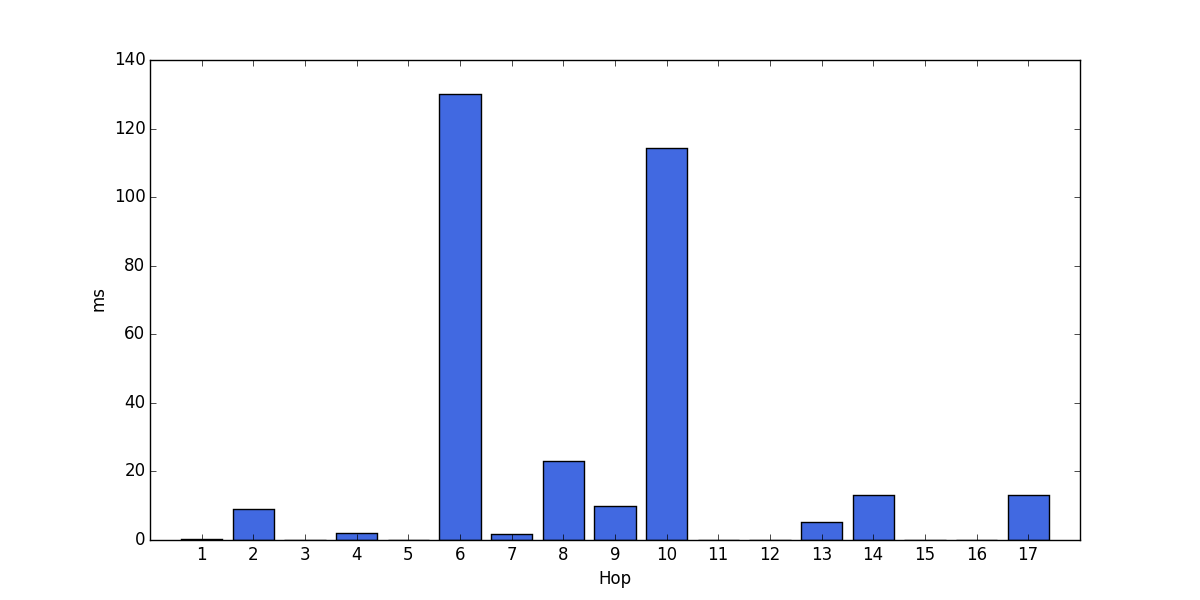
\includegraphics[width=1\textwidth]{data/rtt-tokyo-bar.png}
        \caption{www.u-tokyo.ac.jp - $\Delta$RTT}
        \label{histo:tokyo}
    \end{center}
\end{figure}

\begin{figure}[H]
    \begin{center}
        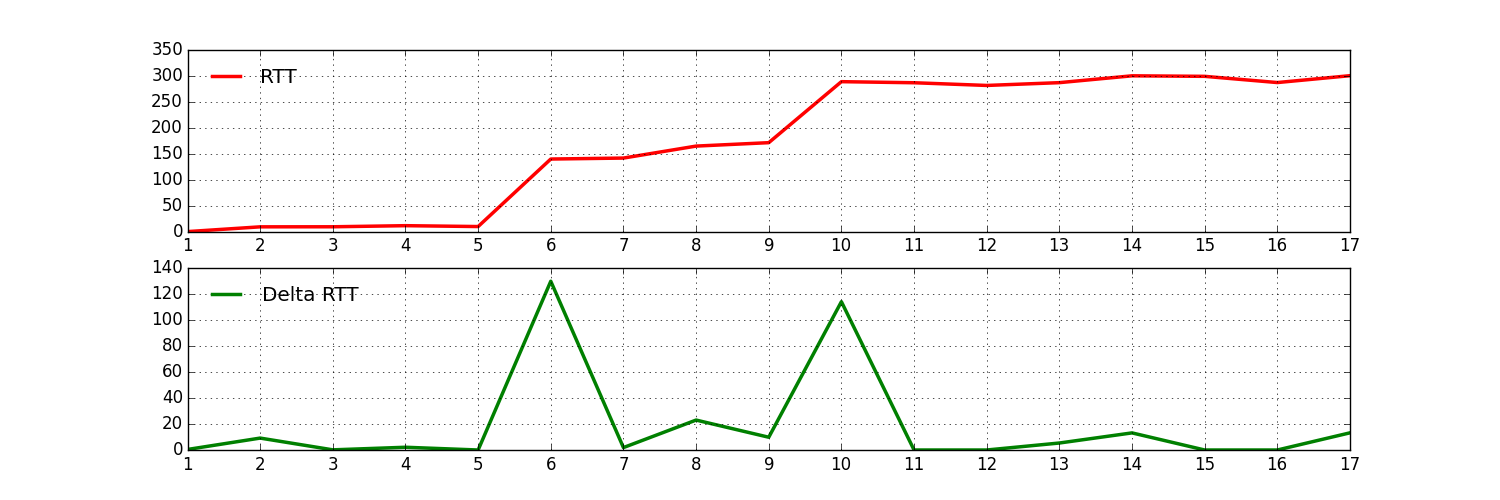
\includegraphics[width=1\textwidth]{data/rtt-tokyo-lines.png}
        \caption{www.u-tokyo.ac.jp - RTT y $\Delta$RTT}
        \label{lines:tokyo}
    \end{center}
\end{figure}

Tanto en la figura \ref{histo:tokyo} como en la figura \ref{lines:tokyo} podemos comprobar los que habiamos notado en la tabla \ref{table:tokyo}. Esto es que tanto el salto 6 como 10 se destacan por sobre el resto. En caso de existir algún enlace submarino seguramente este se correspondería con alguno de estos saltos. Esto lo analizaremos en las siguientes secciones.

\subsubsection{Test de Grubbs}

\subsubsection{Geolocalización}


